\documentclass{article}
\usepackage {inputenc, fullpage, listings, amsmath, graphicx}

\parindent 0pt

\title{%
   CSc 226: Operating Systems (Spring 2022) \\
   \large Written Assignment 2\\
    Alex Holland V00}
    
\date{}

\begin{document}

\maketitle

{\bf Question 1}\\
(a)\\
The sample space associated with the experiment of tossing a fair coin four times where $H=heads$ and $T=tails$ can be represented by the following:\\
$\text{Sample space} (S) = \{HHHH, HHHT, HHTH, HTHH, THHH, HHTT, HTHT,\\ 
HTTH ,THTH, TTHH, THHT, HTTT, THTT, TTHT, TTTH, TTTT\}$\\
$n(S) = 16$

\bigskip
(b)\\
Let A be the event of getting heads on the first flip\\
$A={HHHH, HHHT, HHTH, HTHH, HHTT, HTHT, HTTH, HTTT}$\\
$n(A) = 8$\\
$Pr(A)=\frac{n(A)}{n(S)}=\frac{8}{16}=0.5$

\bigskip
(c)\\
Let B be the even of getting exactly two heads and two tails (in any order):\\
$A={HHTT, TTHH, HTHT, THTH, HTTH, THHT}$\\
$n(B)=6$
$Pr(AB=\frac{n(B)}{n(16)}=\frac{6}{16}=0.375$

\bigskip
(d)\\
$(A \cap B) = \{HHTT, TTHH, HTHT, THTH\}$\\
$Pr(A \cap B) = Pr(A) \times Pr(B) = 0.5 \times 0.375 = 0.1875$


\bigskip
(e)\\
Let $X$ be the number of heads flipped, We can determine the expected value of $X$ by determining $E[x]$\\
Possible values of heads flipped:\\
$X=\{0,1,1,1,1,2,2,2,2,2,2,3,3,3,3,4\}$\\
$n(x) = 16$\\
$E[X] = \frac{\Sigma X}{n(x)}=\frac{0+(4*1)+(6*2)+(4*3)+4}{16}=\frac{32}{16}=2$\\
The expected value of $X$ is 2.

\bigskip
{\bf Question 2}\\
(a)\\
$Pr(H) = \frac{1}{4}$, $Pr(T) = \frac{3}{4}$\\
The expected number of coin tosses required to get heads is:
\begin{equation*} 
\begin{split}
    \frac{1}{Pr(H)} &= \frac{1}{1/4}\\
    &= 4\\
\end{split}
\end{equation*} 

\bigskip
(b)\\
The probability that the number of heads equals the number of tails is:\\
\begin{equation*} 
\begin{split}
    P(x=\frac{n}{2})&={n \choose \frac{n}{2}} p^{\frac{n}{2}}(1-p)^{n-\frac{n}{2}}\\
    &={n \choose \frac{n}{2}}(\frac{1}{4})^{\frac{n}{2}}(1-\frac{1}{4})^{\frac{2n-n}{2}}\\
    &={n \choose \frac{n}{2}}(\frac{1}{4})^{\frac{n}{2}}(\frac{3}{4})^{\frac{n}{2}}
\end{split}
\end{equation*} 

\bigskip
{\bf Question 3}\\
We want to determine a recurrence equation from the following randomized Quicksort Algorithm:
\begin{lstlisting}
Pick a random pivot
Check if the pivot was picked previously 
    If pivot was picked previously, pick a new pivot
    If pivot was is not picked previously, check if it is a good pivot
Complete the partition function
If it is a good pivot, go to a recursive call
If it is a bad pivot, pick another pivot
\end{lstlisting}
The worst case running time when finding a pivot is when we select all the bad pivots before we select a good one. So the worst case running time is $O(n^2)$.\\
So we get that the recurrence equation is:
\begin{equation*} 
\begin{split}
    T(n) &= T(|L|) + T(|G|) + O(n^2)\\
\end{split}
\end{equation*}

Each partition divides the array such that one side has $\frac{n}{4}$ elements and the other has $\frac{3n}{4}$ elements.

\begin{equation*}
\begin{split}
    \frac{n}{4} &\leq |L| \leq \frac{3n}{4}\\
    \frac{n}{4} &\leq |G| \leq \frac{3n}{4}\\
    T(n) &\leq T(n/4)+T(3n/4)+O(n^2)\\
    T(n) &\leq 2T(3n/4)+O(n^2)\\
    \end{split}
\end{equation*}

Masters Theorem
\begin{equation*} 
\begin{split}
    a&=2, \; b=4/3, \; c=2\\
    1 &< log_{4/3}2
    T(n) = \Theta(n^{log_{4/3}2})
\end{split}
\end{equation*}

\bigskip
{\bf Question 4}\\
(a)\\
\begin{equation*} 
\begin{split}
    h(k) &= (2k + 5)mod11\\
    h(12)&=(2 \times 12 + 5)mod11\\
    &=29mod11\\
    &=7\\
\end{split}
\end{equation*}
Repeating these calculations for the remaining keys we get:\\
$h(44)=93mod11=5, \; h(13)=93mod11=9, \; h(88)=181mod11=5, \; h(23)=51mod11=7,\\ h(94)=193mod11=6, \; h(11)=27mod11=5, \; h(39)=83mod11=6, \; h(20)=45mod11=1, \\ h(16)=37mod11=4 \; h(5)=15mod11=4$

\begin{center}
    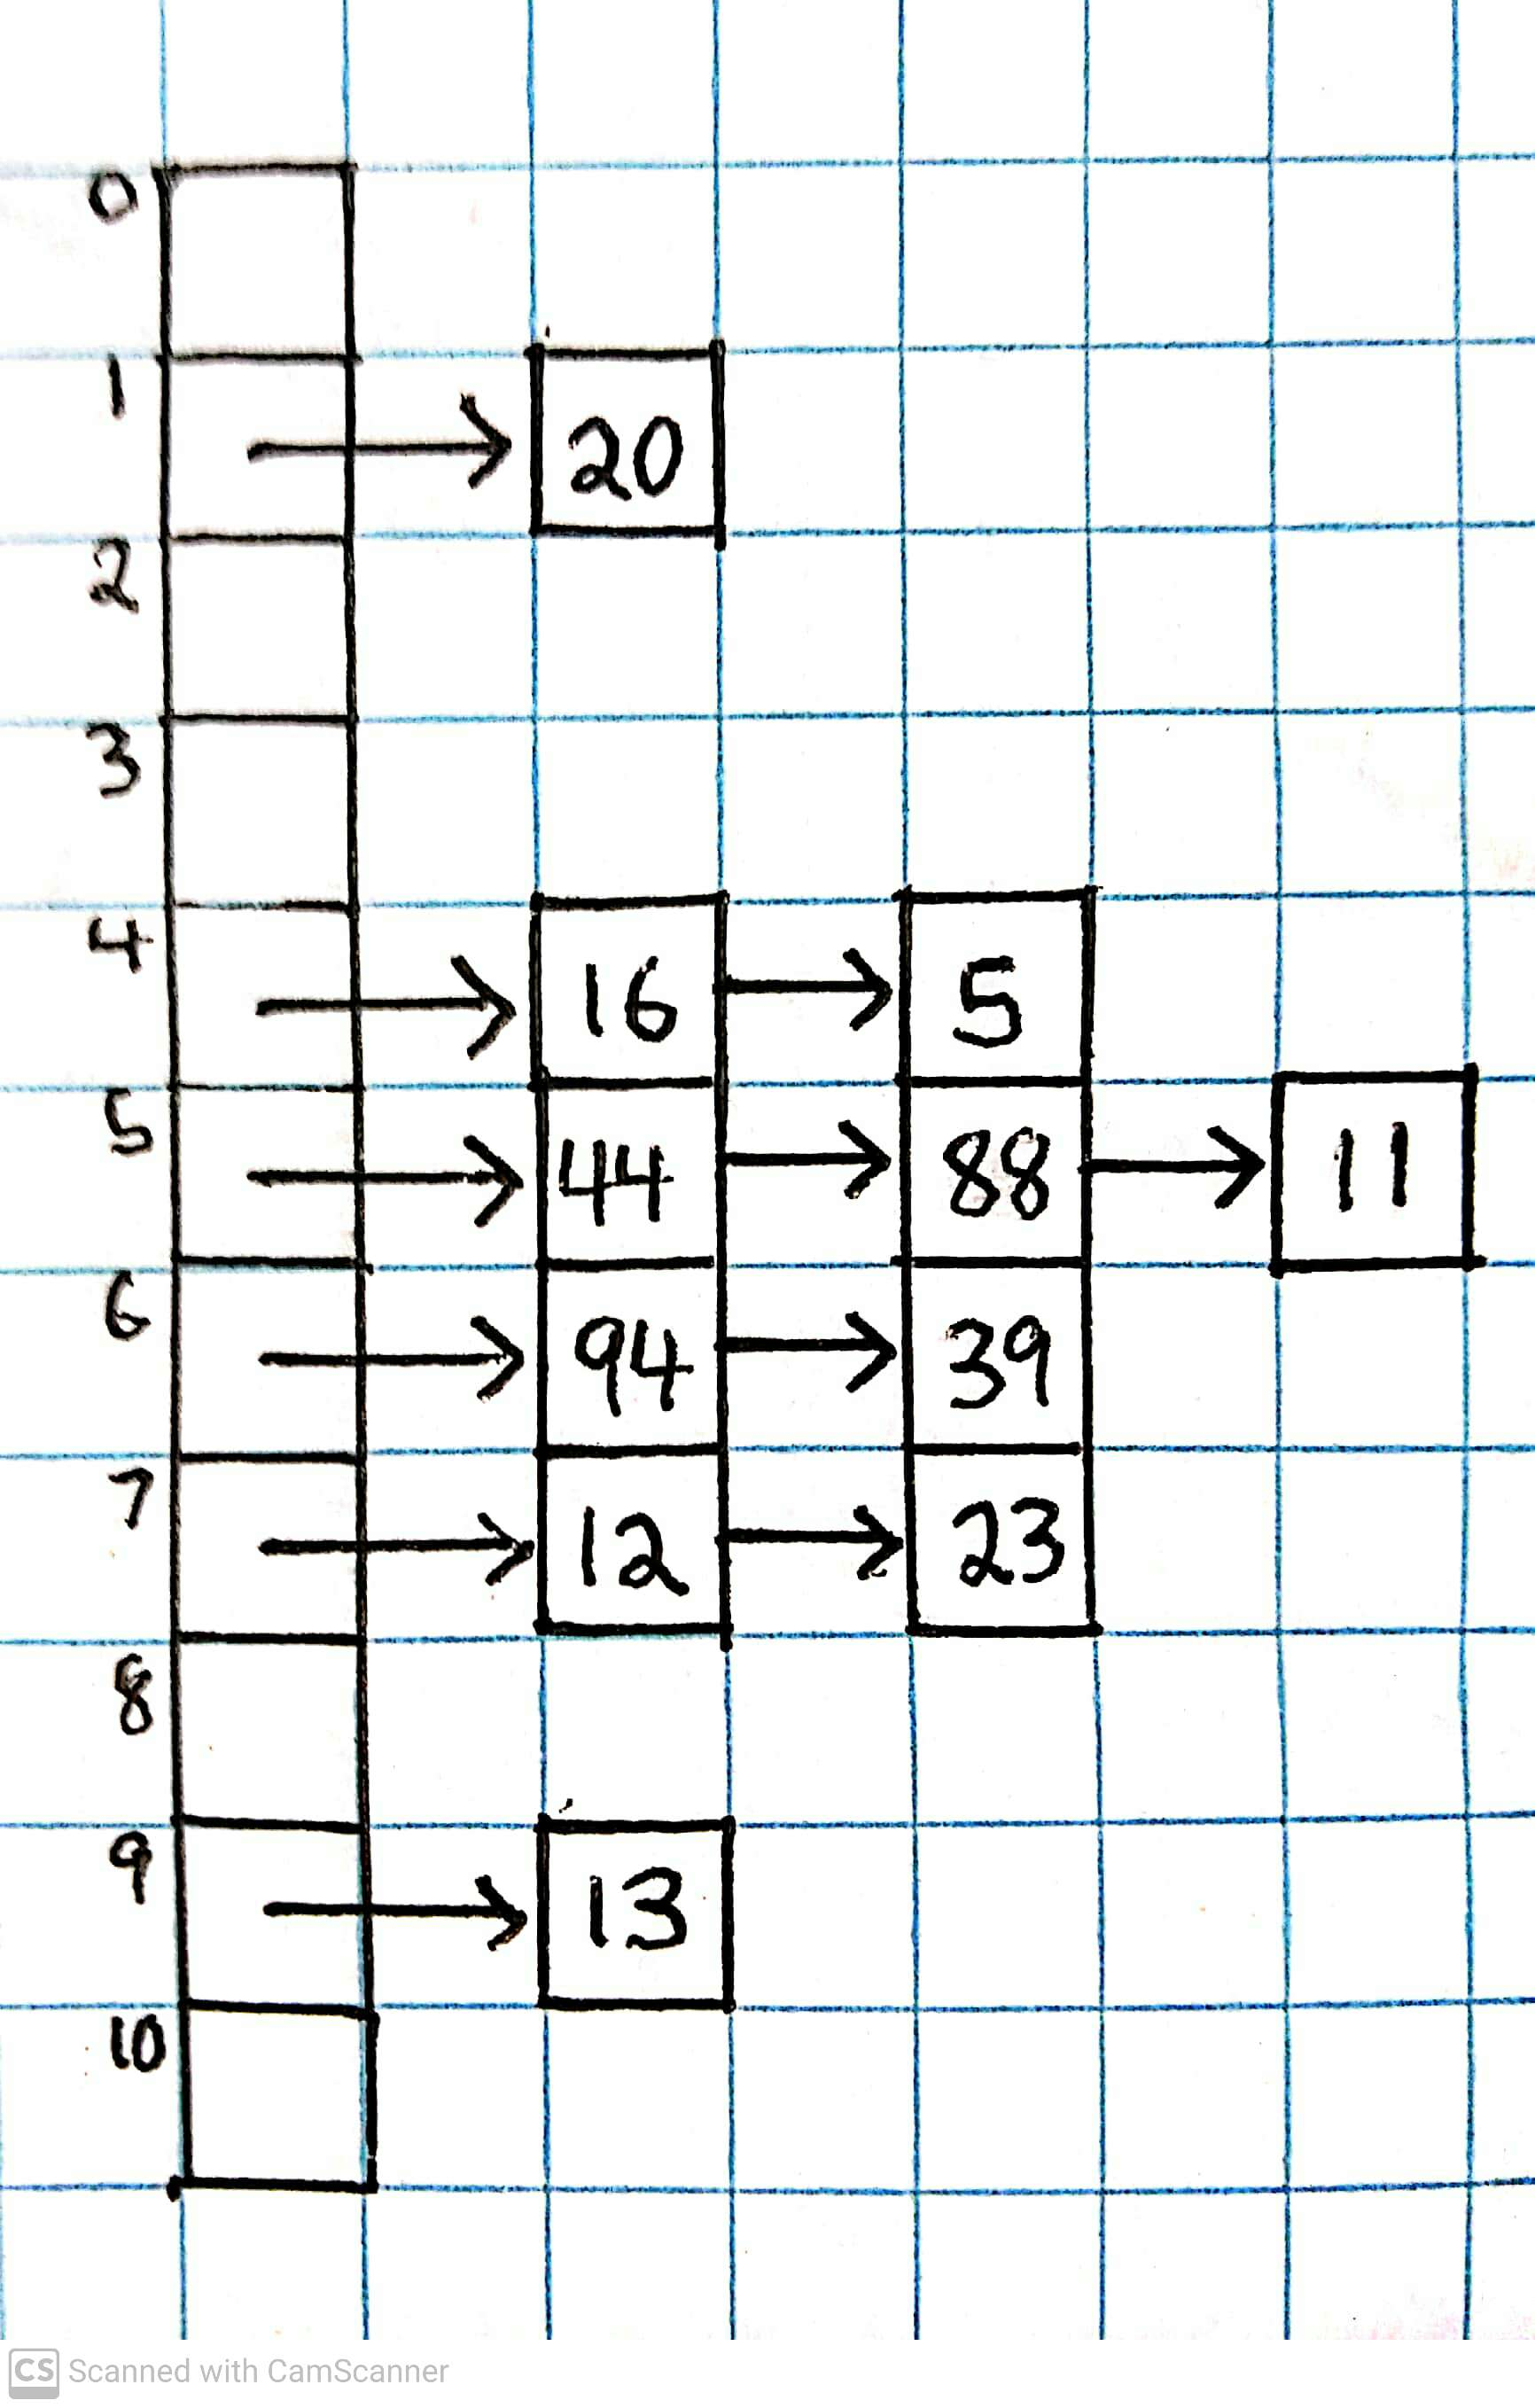
\includegraphics[width=.3\textwidth]{list.jpg}
\end{center}


(b)\\
\begin{equation*} 
\begin{split}
    h(12) &= 29mod11=7\\
    h(44) &= 93mod11=5\\
    h(13) &= 93mod11=9\\
    h(88) &= 181mod11=5 \; \text{occupied}\\
          &= (5+1)mod11=6\\
    h(23) &= 51mod11=7 \; \text{occupied}\\
          &= (7+1)mod11=8\\
    h(94) &= 193mod11=6 \; \text{occupied}\\
          &= (6+1)mod11=7 \; \text{occupied}\\
          &= (7+1)mod11=8 \; \text{occupied}\\
          &= (8+1)mod11=9 \; \text{occupied}\\
          &= (9+1)mod11=10\\
    h(11) &= 27mod11=5 \; \text{occupied}\\
          &= (10+1)mod11=0\\
    h(39) &= 83mod11=6 \; \text{occupied}\\
          &= (6+1)mod11=7 \; \text{occupied}\\
          &...\\
          &= (11+1)mod11=1\\
    h(20) &= 45mod11=1 \; \text{occupied}\\
          &= (1+1)mod11=2\\
    h(16) &= 37mod11=4\\
    h(5) &= 15mod11=4\\
         &= (4+1)mod11=5 \; \text{occupied}\\
         &...\\
         &= (15+1)mod11=3\\
\end{split}
\end{equation*}

\begin{center}
    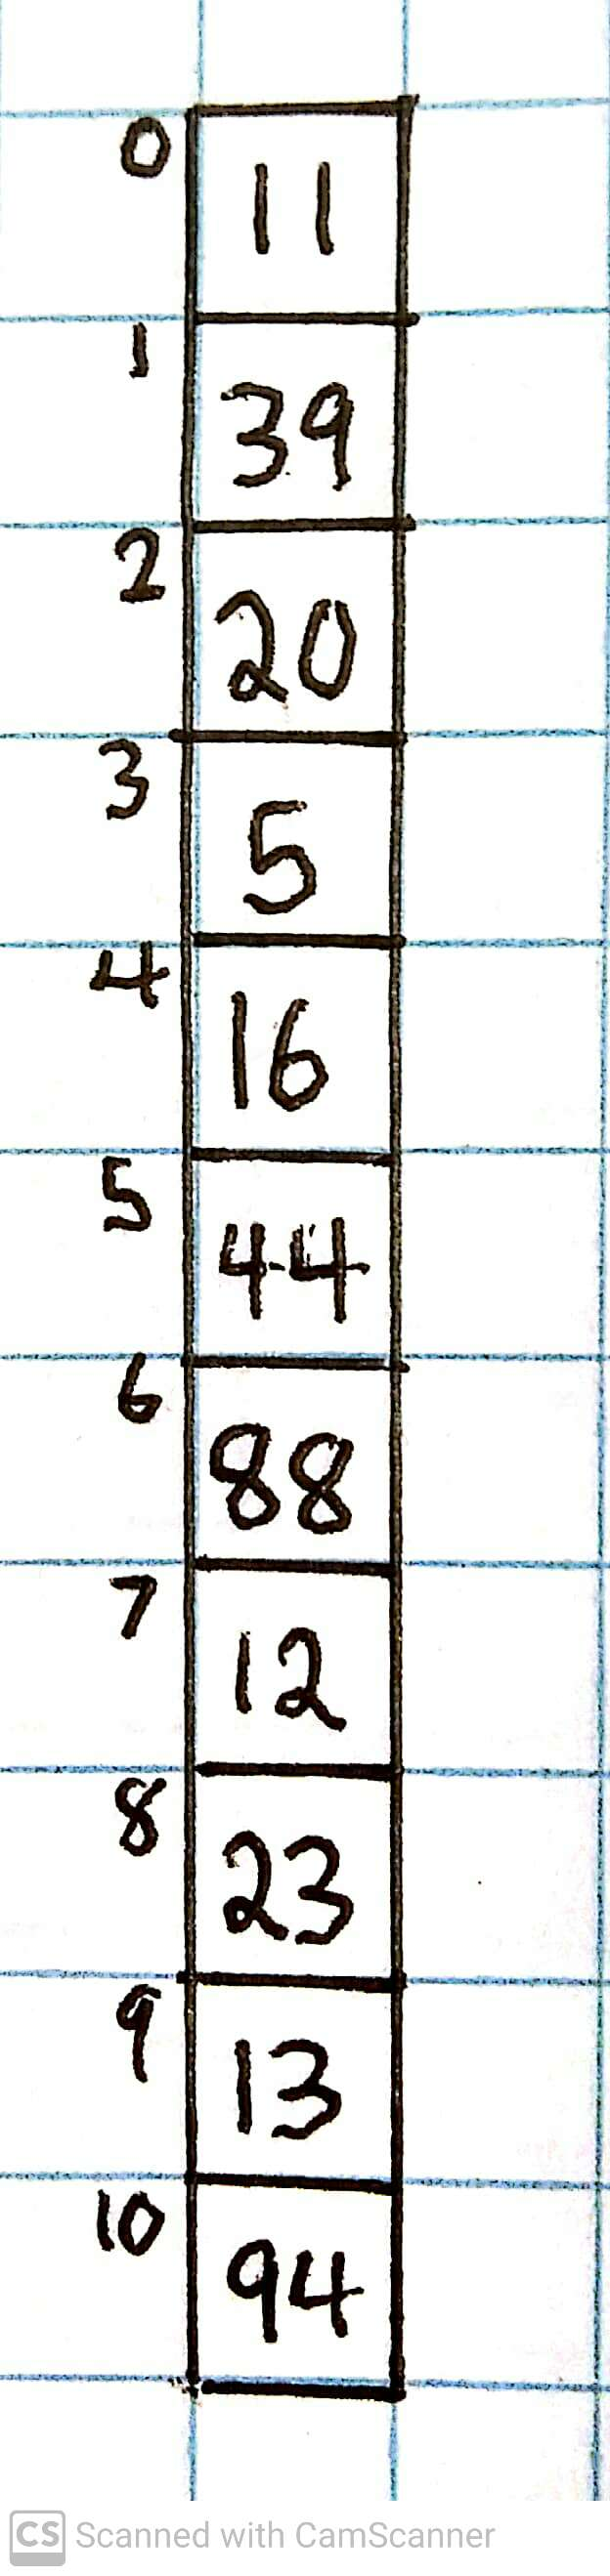
\includegraphics[width=.1\textwidth]{linear.jpg}
\end{center}

(c)\\
\begin{equation*} 
\begin{split}
    h(12) &= 29mod11=7\\
    h(44) &= 93mod11=5\\
    h(13) &= 93mod11=9\\
    h(88) &= 181mod11=5 \; \text{occupied}\\
          &= (5+1^2)mod11=6\\
    h(23) &= 51mod11=7 \; \text{occupied}\\
          &= (7+1^2)mod11=8\\
    h(94) &= 193mod11=6 \; \text{occupied}\\
          &= (6+1^2)mod11=7 \; \text{occupied}\\
          &= (6+2^2)mod11=10 \; \text{occupied}\\
    h(11) &= 27mod11=5 \; \text{occupied}\\
          &= (5+1^2)mod11=6 \; \text{occupied}\\
          &= (5+2^2)mod11=9 \; \text{occupied}\\
          &= (5+3^2)mod11=3\\
    h(39) &= 83mod11=6 \; \text{occupied}\\
          &= (6+1^2)mod11=7 \; \text{occupied}\\
          &= (6+2^2)mod11=10 \; \text{occupied}\\
          &= (6+3^2)mod11=4 \\
    h(20) &= 45mod11=1 \; \text{occupied}\\
    h(16) &= 37mod11=4\\
          &= (4+1^2)mod11=5 \; \text{occupied}\\
          &= (4+2^2)mod11=8 \; \text{occupied}\\
          &= (4+3^2)mod11=2\\
    h(5) &= 15mod11=4 \; \text{occupied}\\
         &= (4+1^2)mod11=5 \; \text{occupied}\\
         &= (4+2^2)mod11=8 \; \text{occupied}\\
         &= (4+3^2)mod11=2 \; \text{occupied}\\
         &= (4+4^2)mod11=9 \; \text{occupied}\\
\end{split}
\end{equation*}
At this point the method fails because no empty slot is found.
\begin{center}
    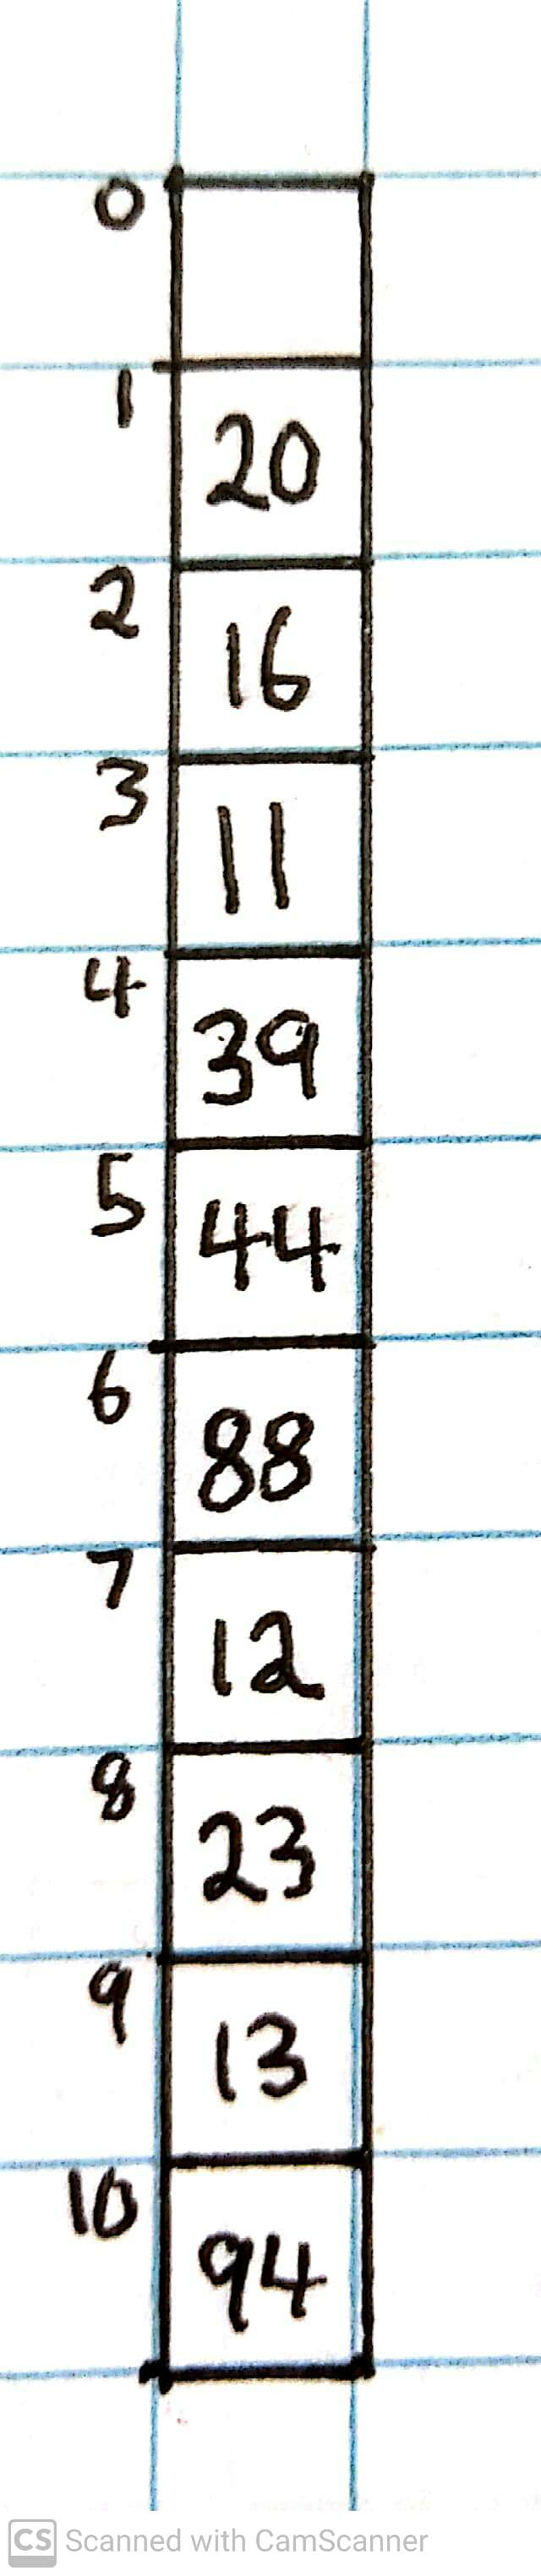
\includegraphics[width=.1\textwidth]{quadratic.jpg}
\end{center}

(d)\\
\begin{equation*} 
\begin{split}
    h(12) &= 7\\
    h(44) &= 5\\
    h(13) &= 9\\
    h(88) &= (h(88) + 1*h'(88))mod11=8\\
    h(23) &= (h(23) + 1*h'(23))mod11=1\\
    h(94) &= 6\\
    h(11) &= (h(11) + 1*h'(11))mod11=8 \; \text{occupied}\\
          &= (h(11) + 2*h'(11))mod11=0\\
    h(39) &= (h(39) + 1*h'(39))mod11=9 \; \text{occupied}\\
          &= (h(39) + 2*h'(39))mod11=1 \; \text{occupied}\\
          &= (h(39) + 3*h'(39))mod11=4\\
    h(20) &= (h(20) + 1*h'(20))mod11=2\\
    h(16) &= (h(16) + 1*h'(16))mod11=5 \; \text{occupied}\\
          &= (h(16) + 2*h'(16))mod11=3\\
    h(5)  &= (h(5) + 1*h'(5))mod11=3 \; \text{occupied}\\
          &= (h(5) + 2*h'(5))mod11=10\\
\end{split}
\end{equation*}

\begin{center}
    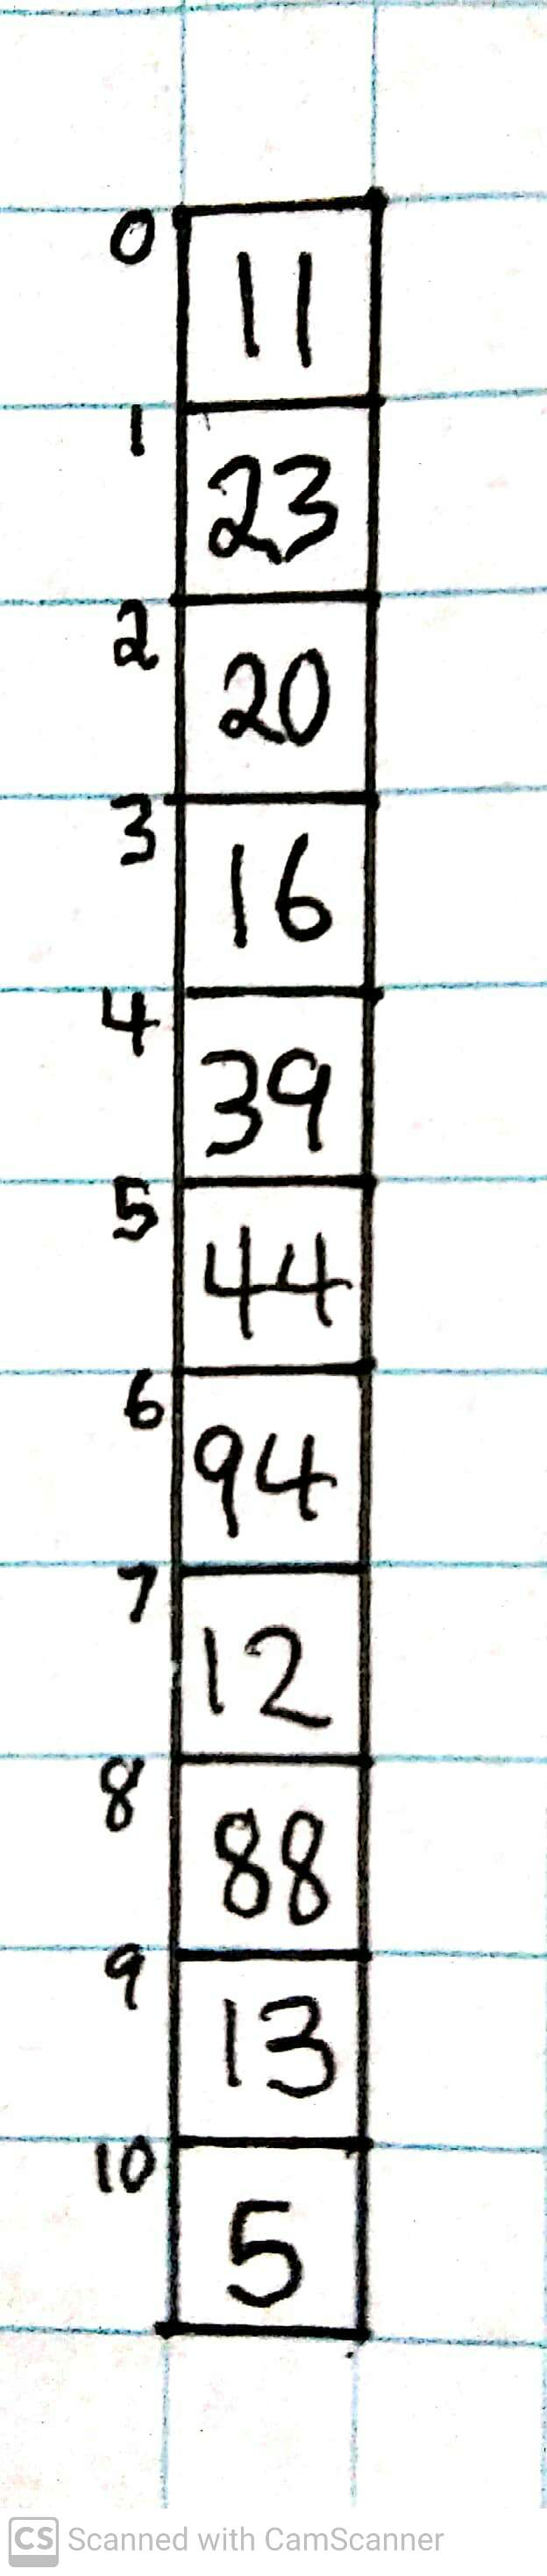
\includegraphics[width=.1\textwidth]{double.jpg}
\end{center}

{\bf Question 5}\\
In this question we refer to the laod factor $\alpha$ as $\frac{n}{m}$ where $n=$number of keys, $m=$number of positions in the table.\\

\smallskip
Running time for successful searches:\\
When a successful search is done on a chaining scheme with unsorted lists the complexity is $\Theta(1+\alpha)$.The worst case scenario happens when the whole list is traversed to locate an element in the list. In the case of the sorted list; the length is still the same. Thus, the running time for a successful searches is $\Theta(1+\alpha)$.\\

Running time for unsuccessful searches:\\
The time complexity for unsuccessful searches of unsorted lists with chaining scheme is $\Theta(1+\alpha)$. The running time of unsuccessful searches proportionally increases with the length of the list. Thus, the running time for an unsuccessful search must also be $\Theta(1+\alpha)$.\\

Running time for insertions:\\
Insertions on a chaining scheme with unsorted lists is always placed at the head of the list, so the running time is $\Theta(1)$. Since Prof. Marley has modified the chaining scheme to use sorted list, an appropriate place to insert the element must be found in the list before insertion. The running time of inserting into a chaining scheme with sorted lists is $\Theta(1+\alpha)$.\\

Running time for deletions:\\
In order for a deletion to be made with a chaining scheme using unsorted lists, the element must be searched for in the list. This means the running time must be the same as the running time of searching. Therefore, the running time for deletions is $\Theta(1+\alpha)$.
\end{document}
